\chapter{HPC MultiBench}
\label{ch:hpc-multibench}

\textbf{This chapter is now complete - but wasn't in the first three chapter draft submission!}

% Having implemented the Rust translation of the HPCCG codebase, the next step is to characterise its performance. This is typically done by running many tests across a wide variety of configurations and problem sizes to understand how the program scales across these metrics.

HPC MultiBench is a tool to generate and run HPC batch compute jobs for performance comparison via Slurm from a convenient YAML configuration file. It can be thought of as ``a Swiss army knife for comparing programs on HPC resources''. This chapter will first discuss the motivation and use case for the tool, then go into technical detail about its design and implementation. Next, it will provide a concrete demonstration of its utility in an example use case, quickly constructing replication studies, by confirming the results of Moran and Bull's paper ``Emerging technologies: Rust in HPC'' \cite{moranEmergingTechnologiesRust2023}. Finally, the chapter will conclude with thoughts from an industry review of the tool by two PhD candidates working in the High Performance and Scientific Computing Group at Warwick.

\section{Motivations}
\label{sec:hpc-multibench-motivation}

Manually spawning and aggregating the metrics from many similar jobs with different configurations is tedious. It is a repetitive and time-consuming process, and as such discourages duplicating results for statistical confidence -- despite being susceptible to human error. However, it is a common task in workflows for designing High-Performance Computing software, as it provides critical metrics to characterise application performance.

Consider a single trial comparing the performance of two programs across eight problem sizes, with eight different thread counts per problem size. In total, this requires 128 program runs. Re-running this trial five times for statistical confidence requires 640 program runs, which is an untenably large number of jobs to dispatch manually. Currently, there are two approaches to this problem: either ignore statistical confidence and manually spawn many jobs, or create an application-specific script to submit the jobs. Both of these approaches are time-consuming, either manually submitting the jobs or writing and debugging the custom script. As a result of this, this step can form a bottleneck in certain workflows.

However, this process of running and aggregating jobs is very similar between performance trials for different programs, meaning it is possible to create a program to automate the process. This combination of being both time-consuming and amenable to automation makes it a very good candidate for building tooling to facilitate it, as it has a good ratio of being high-impact to requiring achievable programming effort.

\section{Existing tools}
\label{sec:hpc-multibench-existing-tools}

As High-Performance Computing is an active research space, there are a number of existing tools which also act as a wrapper around Slurm, as shown in Table \ref{tab:hpc-multibench-existing-tools}. However, none of these tools appear to provide first-class support for this particular use case.

% TODO: Check all tables have bold headings
% TODO: Consider citing GitHub on tool names and papers on tool descriptions?
\begin{table}[H]
    \caption{Existing tools which provide wrappers for Slurm.}
    \label{tab:hpc-multibench-existing-tools}
    \begin{tabular}{|p{0.2\linewidth}|p{0.8\linewidth}|}
    \hline
    \textbf{Tool name}  & \textbf{Tool description} \\ \hline\hline
    slurmR     & ``A lightweight wrapper for Slurm'' \cite{gvegayonJournalOpenSource}, which provides a framework to distribute computation of programs written in the R language across compute clusters, particularly in the field of bio-statistics. \\ \hline
    targets    & ``A Make-like pipeline tool for statistics and data science in R'' \cite{landauTargetsPackageDynamic2021}, which orchestrates processing of programs written in R, providing caching capabilities to avoid re-running unchanged parts of the pipeline. \\ \hline
    batchtools & ``Provides an implementation of a Map-like operation to define and asynchronously execute jobs on a variety of parallel backends'' for the R programming language \cite{langBatchtoolsToolsWork2017}. \\ \hline
    ClusterMQ  & ``[An R package] to send function calls as jobs on a computing cluster with a minimal interface'' \cite{schubertClustermqEnablesEfficient2019}. \\ \hline
    \end{tabular}
\end{table}

From this table we can see that a number of tools exist as wrappers for Slurm for scientific computing workflows. However, these tools are generally focussed on orchestrating High-Performance Computing resources to run scientific computing programs, often in the R programming language, rather than providing a mechanism to run and compare the performance of programs in arbitrary languages. Our research did not identify any existing tools which directly compete with the purpose of HPC MultiBench.

\section{Design and implementation}
\label{sec:hpc-multibench-design}

The HPC MultiBench tool started as utility for personal use to facilitate performance measurements, which then later turned into a production-ready tool. As such, the design was guided by the functionality required by the author to conduct such measurements. As such, the identified goals of the tool are:

\begin{enumerate}
    \item Run programs on High-Performance Computing resources across a range of configurations
    \item Extract numerical metrics from program runs
    \item Re-run programs and aggregate their metrics for statistical confidence in results
    \item Plot graphs showing metric trends over configurations
    \item Use a YAML configuration file to allow the definition of program runs, their metrics, and resulting plots
    \item Render an interactive user interface without an X-forwarded graphical connection
\end{enumerate}

\subsection{User interface}
\label{sec:hpc-multibench-ui}
A key design goal of the project was providing an interactive user interface, which can run on remote machines without requiring setup such as configuring X-forwarding. This was motivated by the fact most High-Performance Computing resources are accessed over an SSH connection, which may be proxied through other servers. To mitigate this, X-forwarded graphical applications can be flaky or have very high latency. As a result of this, the tool was designed to have a simple command line interface, including a mode to render results interactively in the terminal without requiring X-forwarding.

The HPC MultiBench command-line user interface is designed to be familiar to users of existing tools, such as the performance profiler \texttt{perf}. Much like \texttt{perf}, it provides two verb subcommands \texttt{record} and \texttt{report}. The \texttt{record} command asynchronously dispatches experimental runs via Slurm, and the \texttt{report} command aggregates and presents an analysis of the results of this runs.

In addition to these, the \texttt{interactive} subcommand uses the Textual \cite{TextualizeTextual2024} library to render an interactive user interface for dispatching and analysing runs entirely in the terminal. Figure \ref{fig:hpc-multibench-line-plotext-2} shows a screenshot of the interactive mode user interface with graph plotting capabilities, and more can screenshots be found in the documentation website gallery page \url{https://edmundgoodman.co.uk/hpc-multibench/gallery.html}.

\begin{figure}[H]
    \centering
    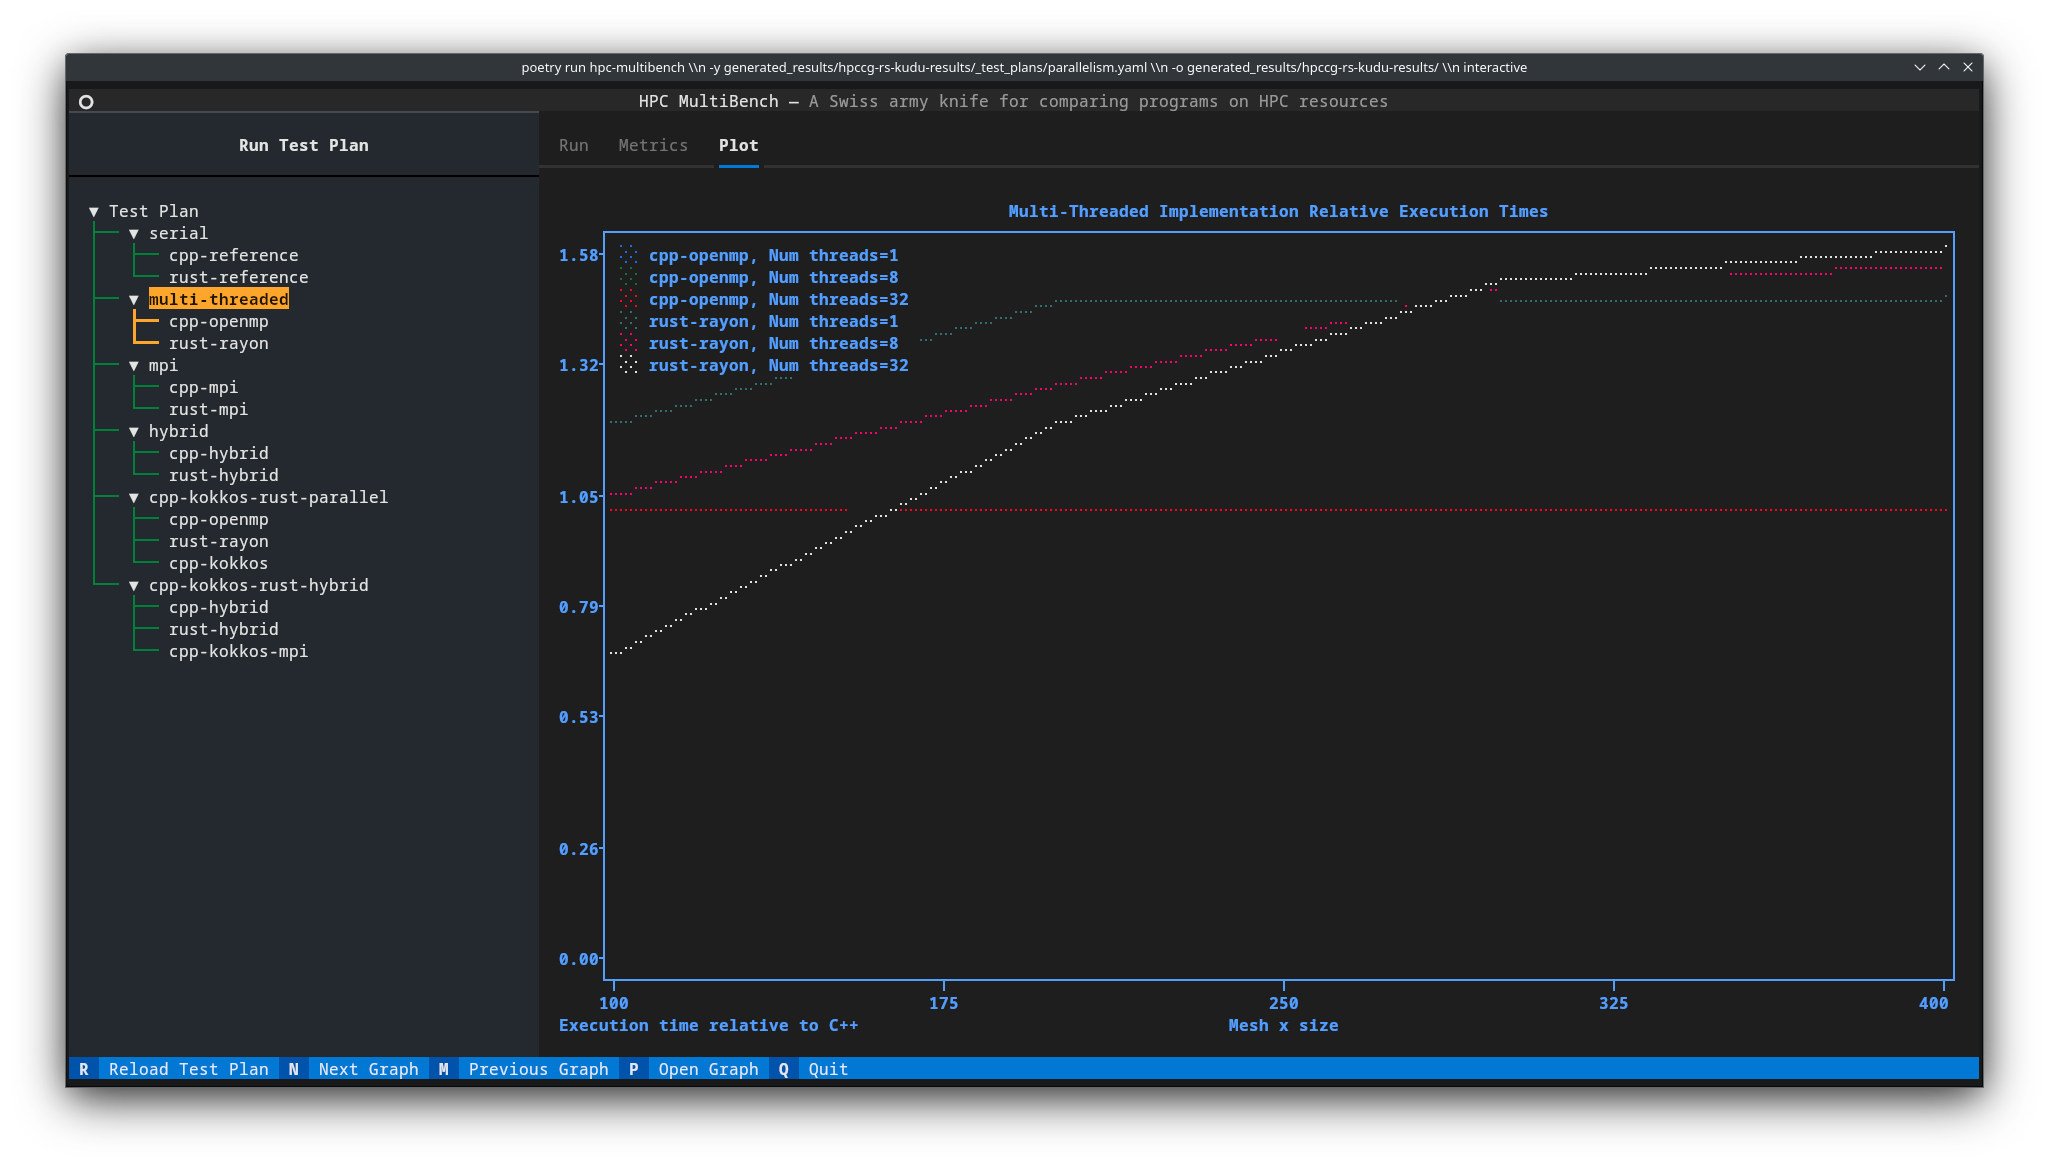
\includegraphics[width=\textwidth]{images/4_tooling/interactive_screenshots/hpc-multibench-line-plotext-2.png}
    \caption{A screenshot of the interactive mode user interface plotting a line graph, rendered entirely in the Terminal.}
    \label{fig:hpc-multibench-line-plotext-2}
\end{figure}

\subsection{Configuration file}
\label{sec:hpc-multibench-configuration-design}

The YAML schema of the HPC MultiBench is the key abstraction which drives its ergonomics and simplicity to use. Since the problem of running, aggregating metrics about, and simple analysis of programs is similar across many use cases, it is possible to create a domain-specific configuration language which expresses the majority of the functionality required. In order to maintain the simplicity, and hence usability, of this abstraction, a minority of complex functionality is not supported. However, mechanisms such as exporting run data for further analysis are provided to mitigate this issue. As discussed in the industry review in section \ref{sec:hpc-multibench-industry-review}, the design of the YAML schema was praised as effectively and ergonomically expressing common functionality.

Structurally, the YAML schema describes a \textit{test plan}, which is composed of two sections. Firstly, \textit{run configurations}, which describe how to run different versions of the program to compare on the computer resource. Secondly, \textit{test benches}, which describe which run configurations to compare, how many statistical re-runs to perform, what should be varied in the course of the experiment, along with the metrics to extract and the analysis to visualise.

The values varied over the course of the experiment are described by a \textit{test matrix}, inspired by continuous integration configuration files to guarantee functionality across many machines. This allows expressing the cross product of two variables through adjacent items, and multiple variables changing independently, through tuple keys. The \textit{metrics} to be analysed are extracted from the outputs on the Slurm job runs with regex patterns. \textit{derived\_metrics} enhance their capabilities through  meta-programming capabilities within the tool to functionally define metrics in terms of ones matched with regex, whilst retaining correct uncertainty values.

For brevity, an in-depth explanation of all the functionality the YAML schema can express is omitted here, but a more full explanation can be found on the documentation website \url{https://edmundgoodman.co.uk/hpc-multibench/yaml_schema.html}, along with relevant auto-generated documentation of the source code \url{https://edmundgoodman.co.uk/hpc-multibench/reference/yaml_model.html}. In addition to this, an example of a YAML file under this schema for the replication study discussed in section \ref{ssec:hpc-multibench-replication-study} can be found in Appendix \ref{sec:tooling-replication-yaml}.

\section{Implementation}
\label{sec:hpc-multibench-implementation}

% One of the key aspects of the implementation of the tool is the robust parsing of the configuration YAML file. In order to do this, the Pydantic library is used to leverage Python type annotations to extract structured data from a dictionary extracted from the YAML file. This is similar to an object-relational model for databases, constructing a sequence of nested objects representing the state of the configuration file which can then be used natively and type-safely within the rest of the codebase. Finally, this approach makes the parsing logic very explicit, and as such the schema can be understood through the docstring-generated documentation for this ORM available on the documentation website \url{https://edmundgoodman.co.uk/hpc-multibench/reference/yaml_model.html}.

% Having parsed the configuration data, the majority of the application logic refers to the data processing pipeline to create and run the instantations, then extract metrics from and aggregate the results. These data flows are depicted in Figure \ref{}, and are described in more detail in the docstring-generated documentation for the \textit{test bench} class \url{https://edmundgoodman.co.uk/hpc-multibench/reference/test_bench.html}.

% TODO: diagram of data flow

% Implementation of the TUI and plotting functionality

% TODO: Consider merging this with the design section?
% TODO: How do I say that making complex tooling is very hard, but I am really good at python/building tooling so I managed it...
Due to the complexity of the source code composing the tool, many of the details of its implementation are omitted for brevity. This is to allow space to focus on the implementation details of the Rust translation of HPCCG discussed in \Cref{ch:translation}, and the use cases for and industry review of the tool in sections \ref{sec:hpc-multibench-example-use-case} and \ref{sec:hpc-multibench-industry-review} respectively.


\subsection{Developer tooling and documentation}
\label{ssec:hpc-multibench-developer-tooling-documentation}

For any software development project of non-trivial size, it is critical to leverage industry best practices to maximise productivity. Using the \texttt{scc} \cite{boyterBoyterScc2024} tool on the \texttt{src/} directory, HPC MultiBench was measured as 1572 lines of Python excluding blank space and code comments. Applying the COCOMO developer productivity model used by \texttt{scc} and as discussed in \Cref{ch:background}, this is estimated to take 4.18 months to develop, and cost \$43,438 in an average industry setting. Due to the author's experience building such tools, and current occupation as a student, significantly less time and no cost was required to undertake this development.

To ensure that the development was completed on time, best practices such as \texttt{git} for version control were leveraged. In addition to this, more esoteric tooling such as pre-commit hooks to run linters and type checkers, along with continuous integration infrastructure, allowed software bugs to be caught early.

% TODO: Does this show off quite how cool the tool is?
% TODO: Could add screenshot of the auto-generated docs from docstrings
For a software tool to be adopted, users must be able to install it, run it, and apply it to their use cases. As a result of this, documentation is required to explain to users how to perform these steps. As part of its continuous integration infrastructure, HPC MultiBench generates a documentation website generated from markdown and docstrings in the python source code using \texttt{MkDocs-Material} framework \cite{donathSquidfunkMkdocsmaterial2024}, which is then deployed as a static site hosted on GitHub pages. This documentation site can be found at \url{https://edmundgoodman.co.uk/hpc-multibench/}, with a screenshot of the splash page shown in Figure \ref{fig:documentation_splash}.

\begin{figure}[H]
    \centering
    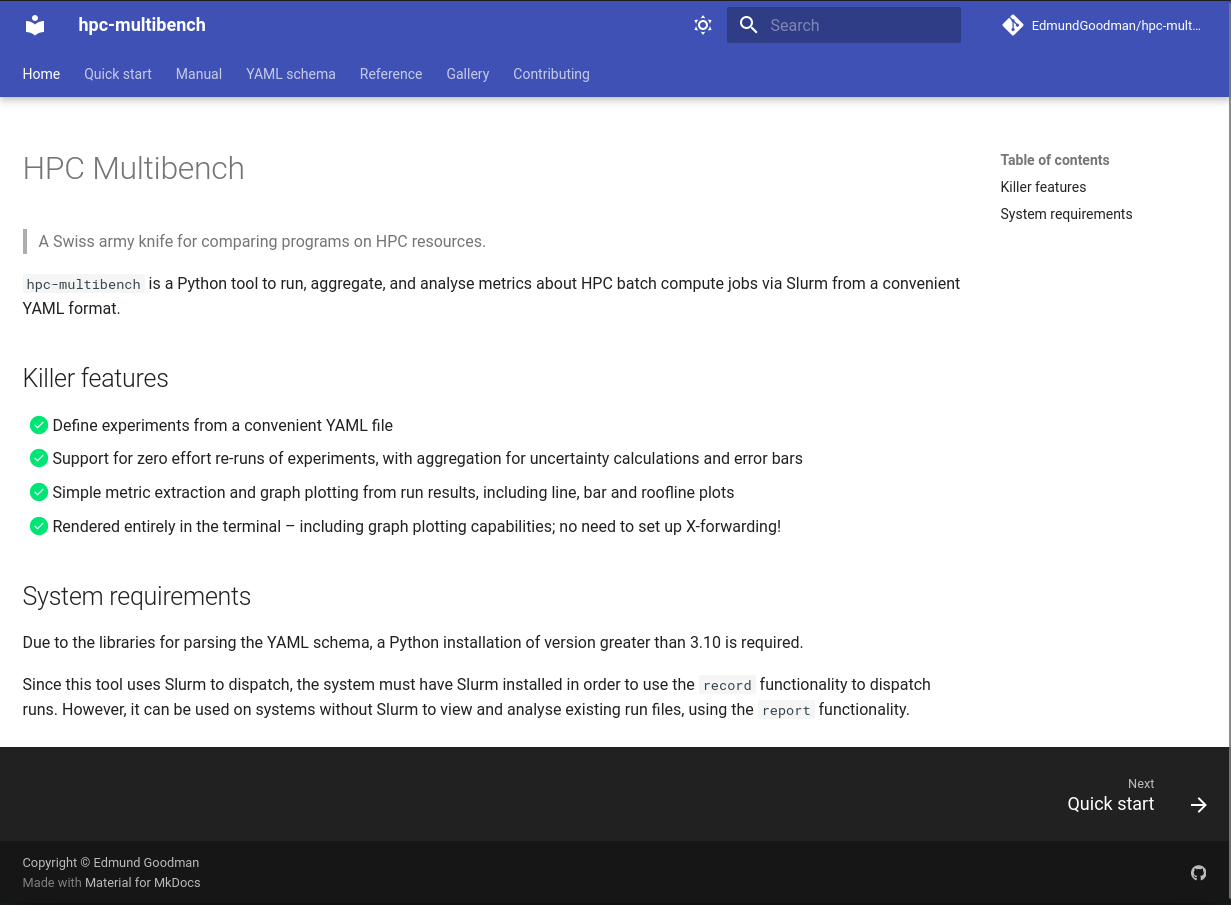
\includegraphics[width=\textwidth]{images/4_tooling/documentation_splash.png}
    \caption{A screenshot of the documentation website splash page for the HPC MultiBench tool, hosted at \url{https://edmundgoodman.co.uk/hpc-multibench/}.}
    \label{fig:documentation_splash}
\end{figure}


\section{Example use case}
\label{sec:hpc-multibench-example-use-case}

As discussed in section \ref{sec:hpc-multibench-motivation}, a key motivation for this tool is streamlining the tedious process of manually running, aggregating, and analysing the results of a large number of program runs to create a statistically confident characterisation of the performance of programs. Since this process is so time-consuming, due to both the process of conducting many runs, and re-writing scripts to aggregate and present the data, it is often not viable to spend time running replication studies of existing work, despite the benefits many benefits this work provides. Beyond the clear use case for this tool of running and analysing original results, which is showcased in full in \Cref{ch:performance}, this tool also makes it possible to very quickly conduct replication studies of existing work in the field.

In his paper ``Shall we Really do it Again? The Powerful Concept of Replication is Neglected in the Social Sciences'', Schmidt introduces replication as ``one of the central issues in any empirical science'', and goes on to define replication studies as ``'' \cite{schmidtShallWeReally2009}. In recent years, the absence of reproducible results in publications has been branded the ``replication crisis'', with Ioannidis publishing a paper title ``Why Most Published Research Findings Are False'' on the basis of a very high rate of non-reproducibility of experimental data \cite{ioannidisWhyMostPublished2005}. Since High-Performance computing relies on many empirical measurements draw conclusions about characteristics of hardware and software, tooling to facilitate reproducibility is clearly desirable.

\subsection{Replication study of ``Emerging technologies: Rust in HPC''}
\label{ssec:hpc-multibench-replication-study}

This section shows the workflow of running a replication study on Moran and Bull's paper ``Emerging technologies: Rust in HPC'' \cite{moranEmergingTechnologiesRust2023}. This paper was selected as the source code is available as a GitHub repo \cite{Lmoran94Eurocc_cfdCFD}, and the paper draws a different conclusion to other existing work such as Constanza et al. \cite{costanzoPerformanceVsProgramming2021}, so replication would either provide confidence in their results, or elucidate any possible reasons for this difference.

As a result of the focussed design goals of the HPC MultiBench tool, the workflow for the replication study facilitated by the HPC MultiBench tool is exceedingly simple, consisting of six short steps -- each of which requires only one terminal command:

\begin{enumerate}
    \item Clone the GitHub repository containing the source code
    \item Add the HPC MultiBench tool as a submodule to the repository
    \item Install the HPC MultiBench tool using \texttt{poetry}
    \item Write a YAML file defining the run configurations and analysis presented in the paper
    \item Use the \texttt{record} command of the HPC MultiBench tool to run the jobs defined by the YAML file
    \item Use the \texttt{report} command of the HPC MulitBench tool to run analyse the results defined by the YAML file
\end{enumerate}

Listing \ref{listing:replication-study-workflow} shows the six terminal commands required to perform these six steps.

% TODO: Consider framing all listings with [linenos,breaklines,frame=single]
% TODO: Submoduling strategy has changed, update to reflect this
\begin{code}
    %TC:ignore
    \begin{minted}{bash}
        git clone https://github.com/lmoran94/eurocc_cfd
        git submodule add https://github.com/EdmundGoodman/hpc-multibench
        cd hpc_multibench && poetry install
        vim ../replication_study.yaml  # The YAML file representing the paper is written here
        poetry run hpc_multibench \
            -y generated_results/eurocc_cfd-kudu-results/ _test_plans/perf_comparison.yaml \
            record
        poetry run hpc_multibench \
            -y generated_results/eurocc_cfd-kudu-results/ _test_plans/perf_comparison.yaml \
            report
    \end{minted}
    %TC:endignore
    \caption{A listing of the six bash commands required to run a full replication study of Moran and Bull's paper ``Emerging technologies: Rust in HPC'' \cite{moranEmergingTechnologiesRust2023}.}
    \label{listing:replication-study-workflow}
\end{code}

The necessary complexity to represent the unique aspects of the results being replicated is encoded in the YAML file, which is shown in Listing \ref{listing:replication-study-workflow} as being written in \texttt{vim}. This is the most involved part of the process, but the abstractions in the design of the YAML schema are designed to make it as simple as possible, whilst still being able to represent most common analyses done by papers.

A full listing of the YAML file for the replication study is provided in Appendix \ref{sec:tooling-replication-yaml}. It is only 190 lines long, much of which can be templated from examples in the tool documentation. This is significantly shorter in line length than the code that would be required to script running all the configurations of the programs, aggregating the results, and plotting graphs for them -- and avoids much of the time spent debugging that would be required for writing such custom scripts. Examples of the original and replicated figures from the paper are shown pairwise in figures \ref{fig:replication_mine_1}, \ref{fig:replication_original_1}, \ref{fig:replication_mine_2}, \ref{fig:replication_original_2}, \ref{fig:replication_mine_4}, and \ref{fig:replication_original_4}.

\newpage

\begin{figure}[H]
    \centering
    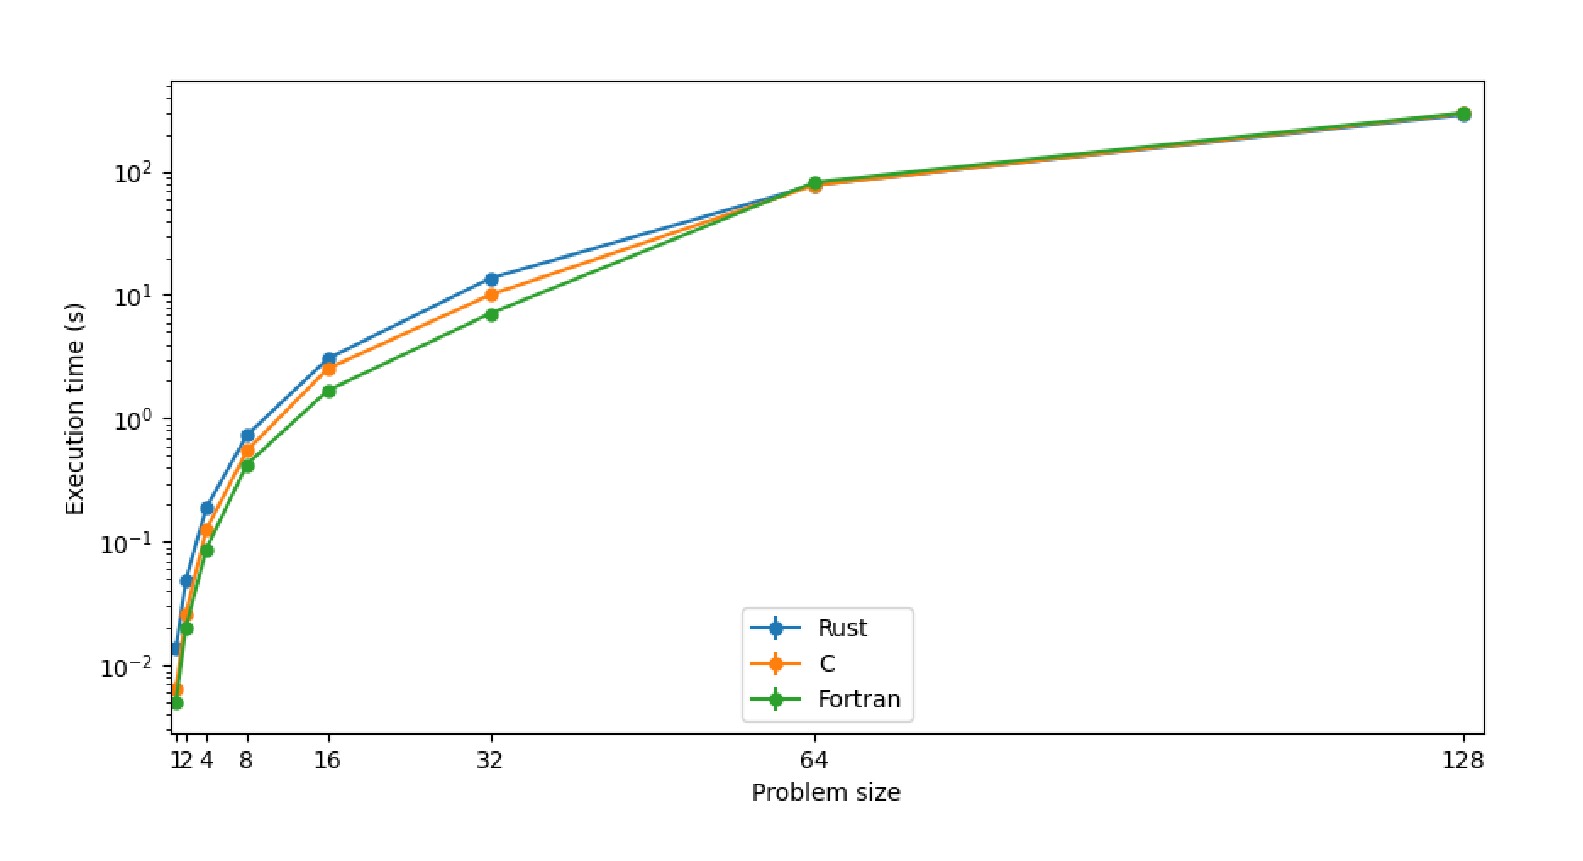
\includegraphics[width=\textwidth]{images/4_tooling/replication_study/replication_original_1.png}
    \caption{A plot comparing total time taken for a serial codebase, from Moran and Bull's paper \cite{moranEmergingTechnologiesRust2023}.}
    \label{fig:replication_original_1}
\end{figure}
\begin{figure}[H]
    \centering
    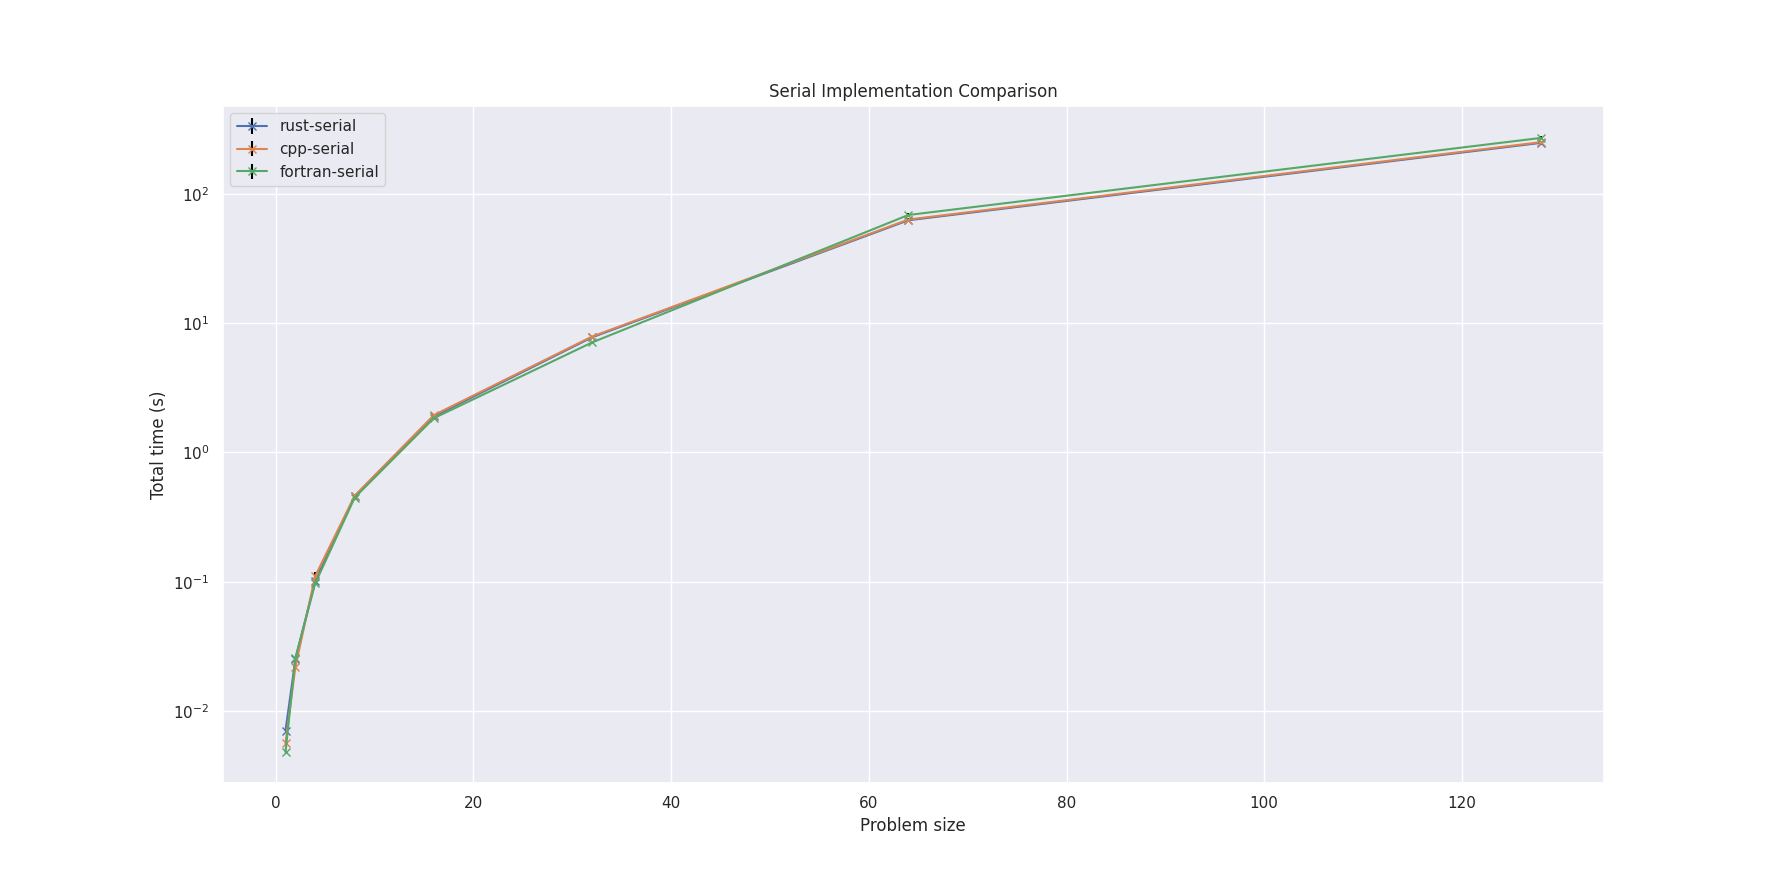
\includegraphics[width=\textwidth]{images/4_tooling/replication_study/replication_mine_1.png}
    \caption{A plot comparing total time taken for a serial codebase, replicated using HPC MultiBench.}
    \label{fig:replication_mine_1}
\end{figure}


\begin{figure}[H]
    \centering
    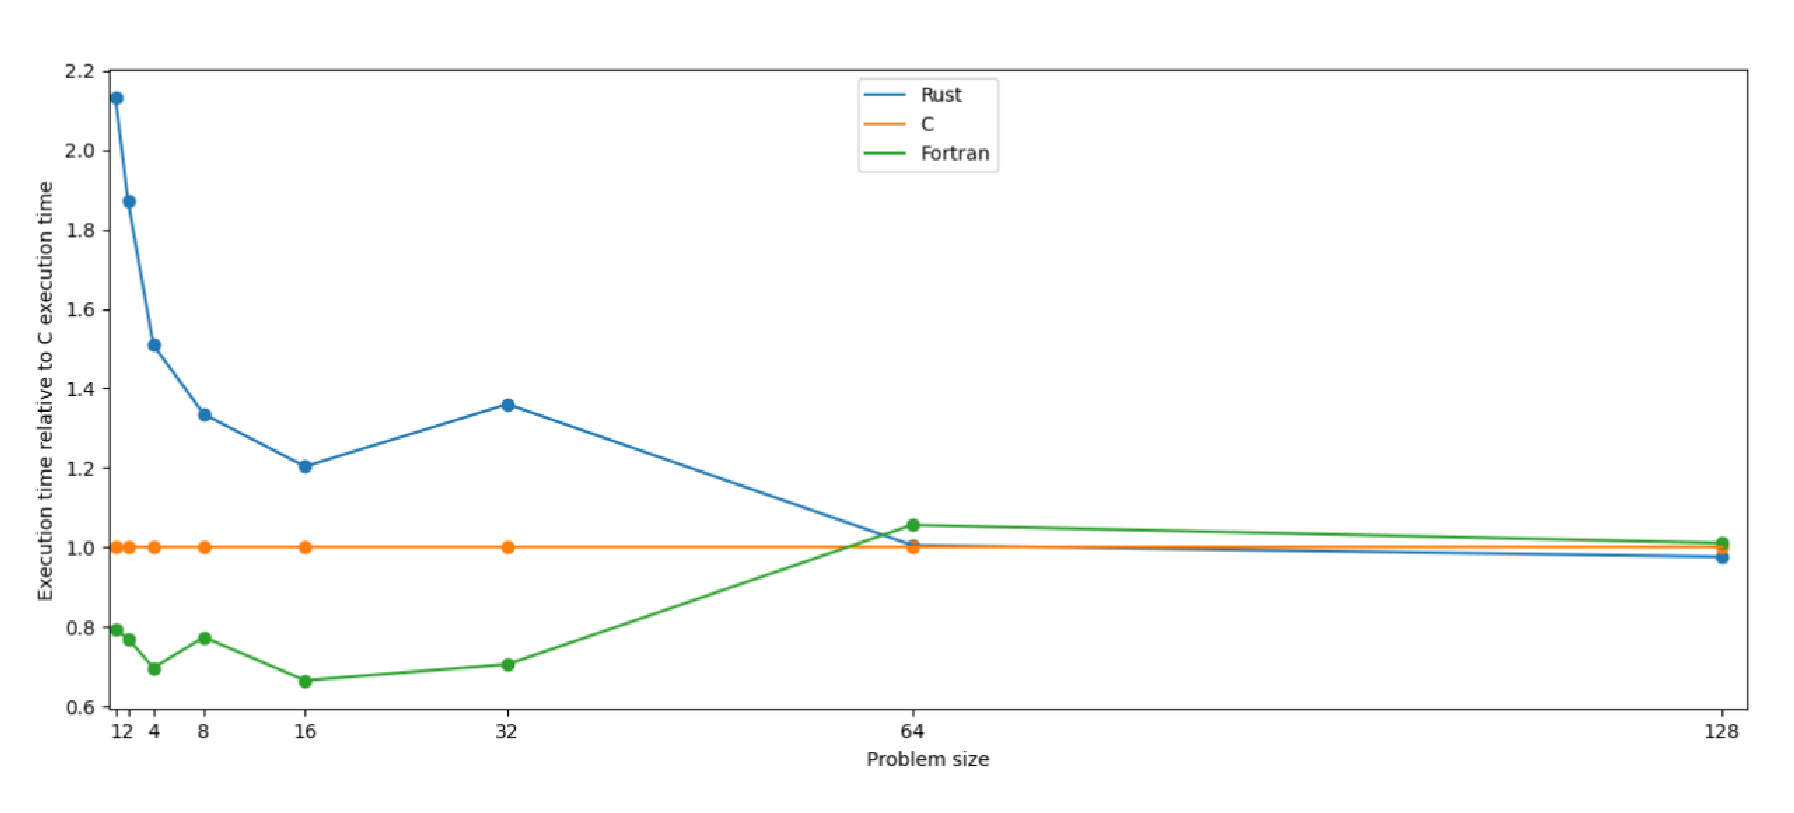
\includegraphics[width=\textwidth]{images/4_tooling/replication_study/replication_original_2.png}
    \caption{A plot comparing serial execution times relative to C++, from Moran and Bull's paper \cite{moranEmergingTechnologiesRust2023}.}
    \label{fig:replication_original_2}
\end{figure}
\begin{figure}[H]
    \centering
    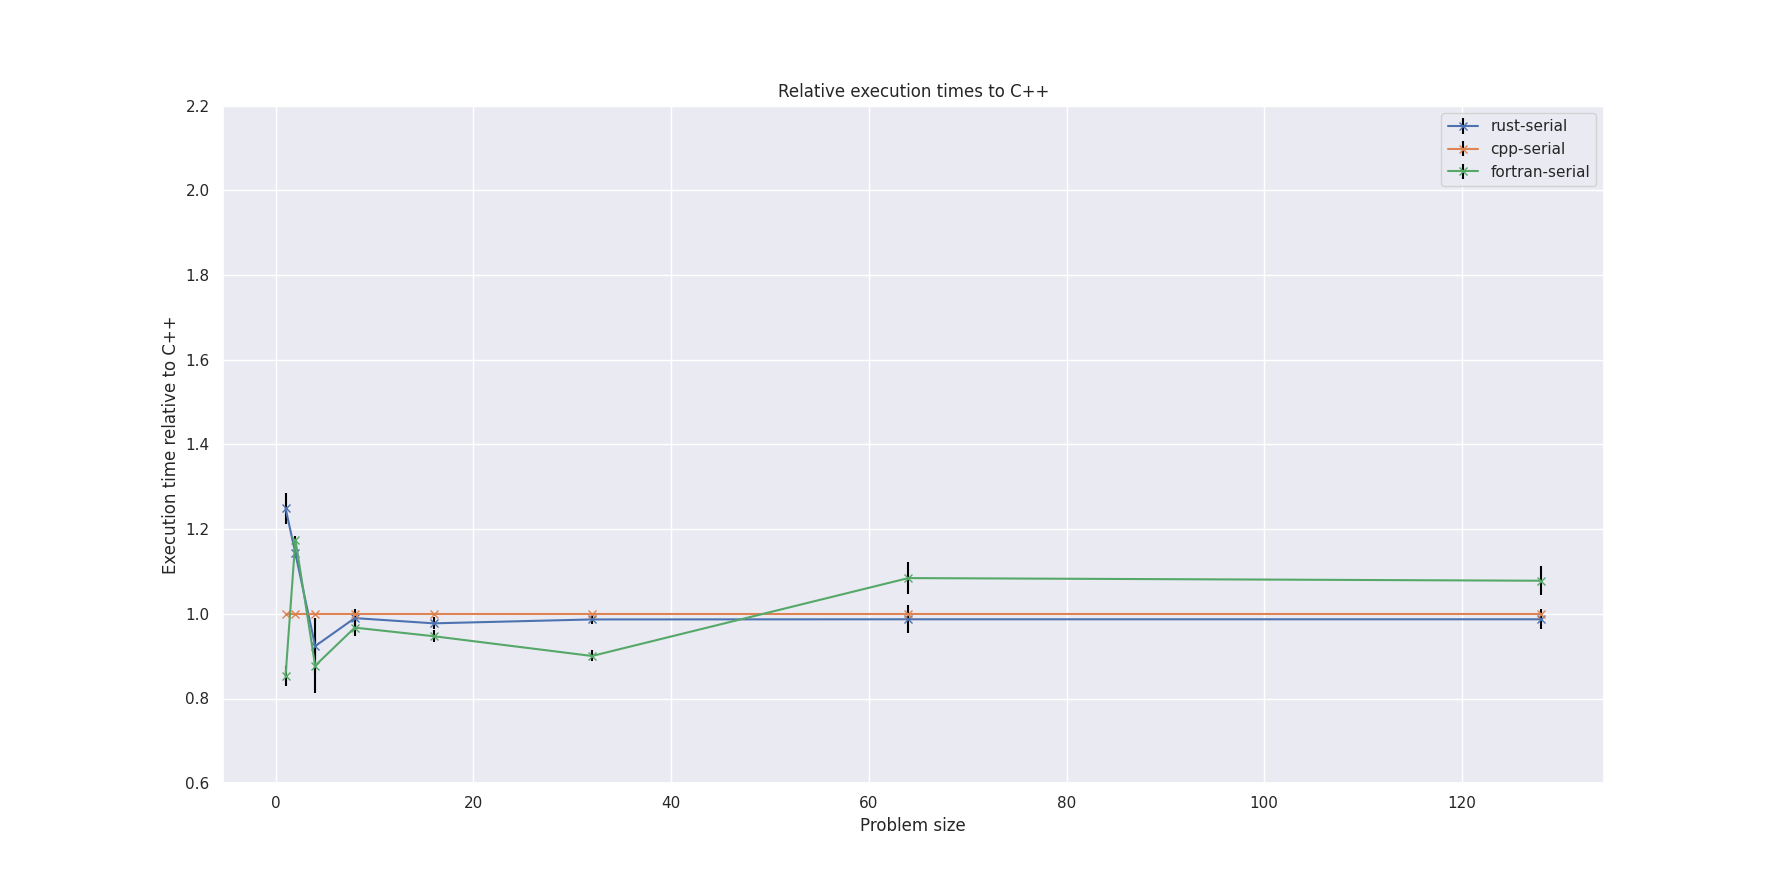
\includegraphics[width=\textwidth]{images/4_tooling/replication_study/replication_mine_2.png}
    \caption{A plot comparing serial execution times relative to C++, replicated using HPC MultiBench.}
    \label{fig:replication_mine_2}
\end{figure}


\begin{figure}[H]
    \centering
    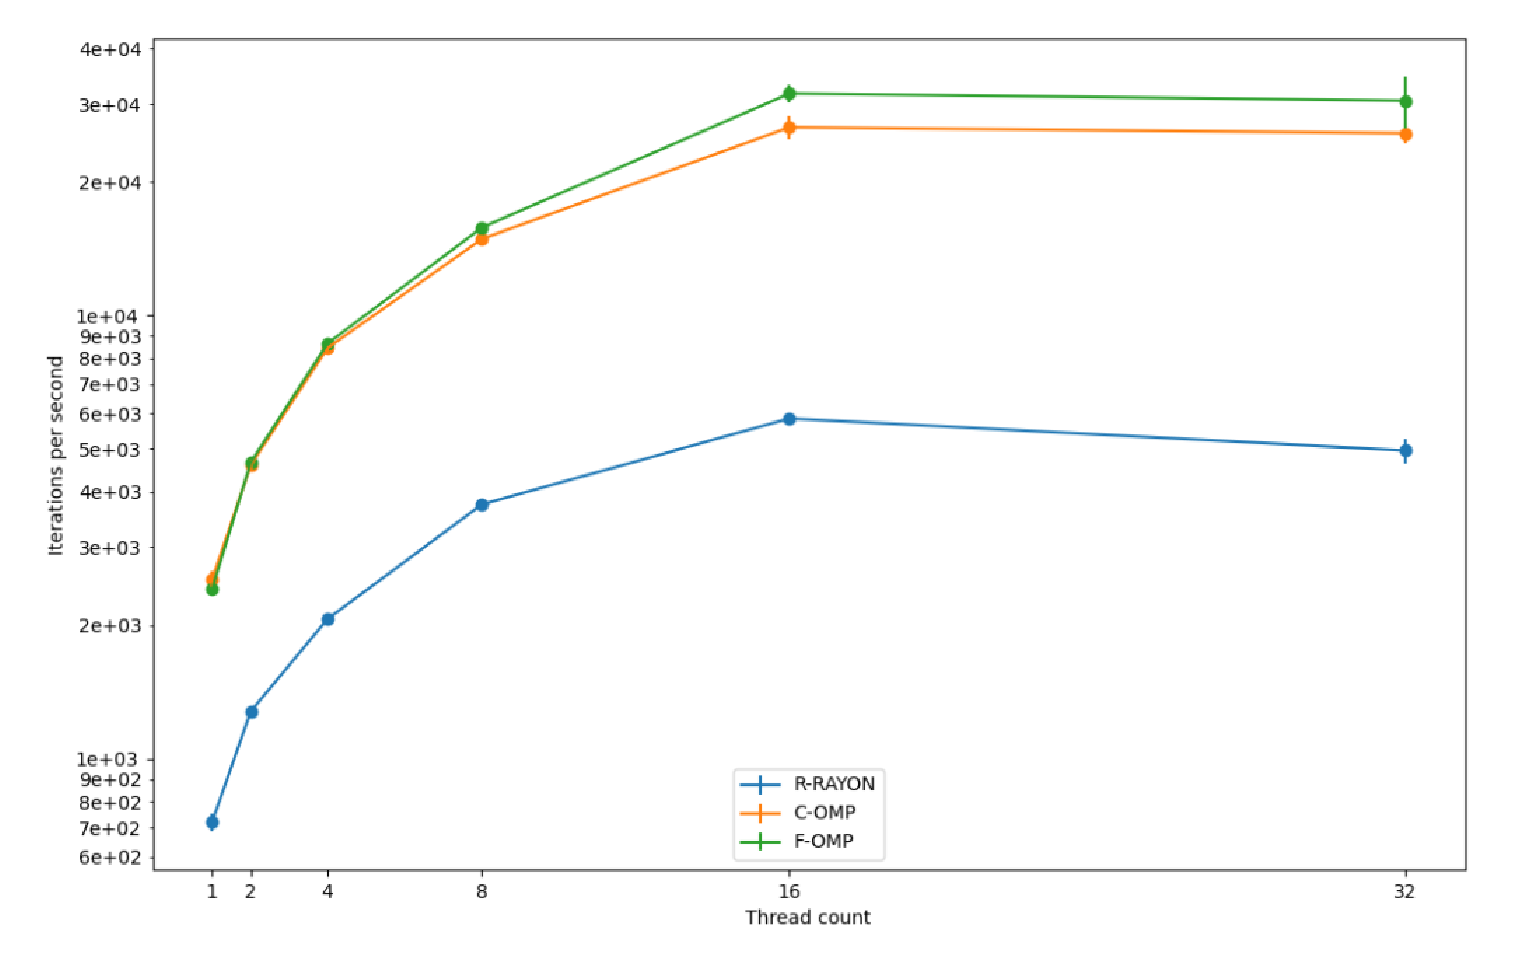
\includegraphics[width=\textwidth]{images/4_tooling/replication_study/replication_original_4.png}
    \caption{A plot showing rate of iterations scaling with the number of threads used, from Moran and Bull's paper \cite{moranEmergingTechnologiesRust2023}.}
    \label{fig:replication_original_4}
\end{figure}
\begin{figure}[H]
    \centering
    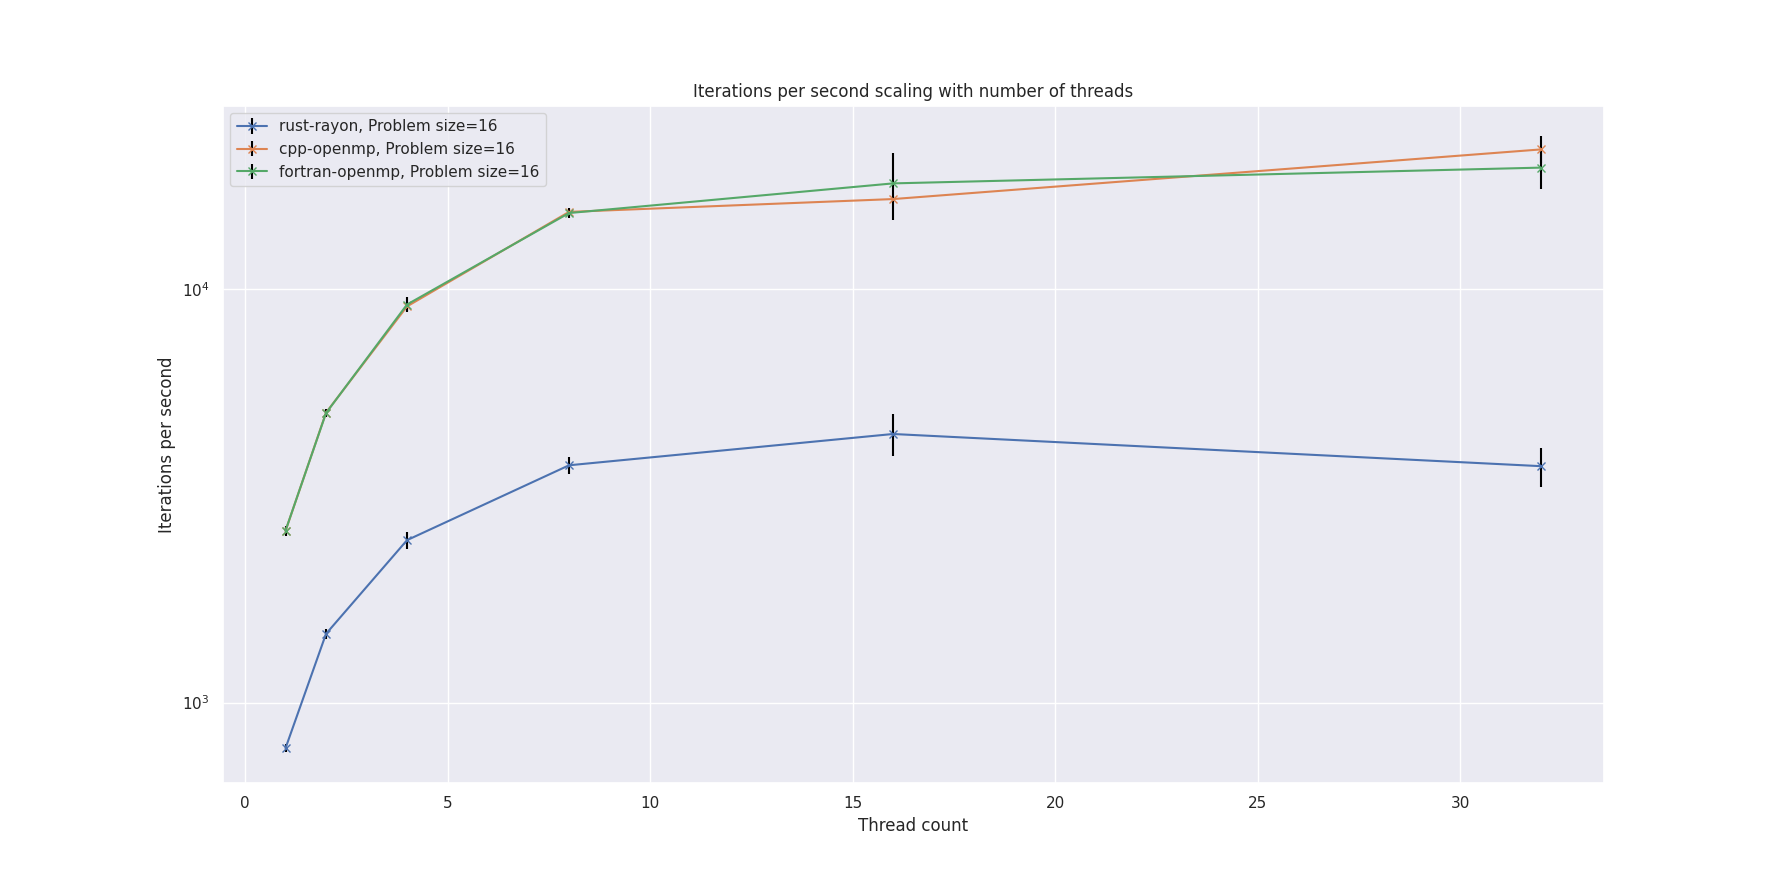
\includegraphics[width=\textwidth]{images/4_tooling/replication_study/replication_mine_4.png}
    \caption{A plot showing rate of iterations scaling with the number of threads used, replicated using HPC MultiBench.}
    \label{fig:replication_mine_4}
\end{figure}


The results of the replication trial broadly match those reported in the paper, with the exception of \ref{fig:replication_mine_4} for small mesh sizes, which could differ as a result of machine noise. The key take-away of this process is the degree to which the HPC MultiBench tool simplifies this critical process in the un-biased review of academic literature, turning a task which would take many hours to do manually into one which only takes about half an hour if the YAML file needs to be created, or just seconds if the YAML file is published with the results.

However, the utility of the HPC MultiBench tool is not limited to conducting replication trials -- it is also incredibly useful for conducting original experiments. However, replication trials best demonstrate the very high reduction in developer time as a result of the tool, by fixing the impact of experimental design.


\section{Industry review}
\label{sec:hpc-multibench-industry-review}

Once development of the HPC MultiBench tool was complete, meetings with two PhD candidates, Toby Flynn and Sam Curtis, both working in the High Performance and Scientific Computing Group at Warwick were organised. These meeting served review the tool, help understand how it fits into the existing landscape, and collect suggestions for future features.

In both meetings, the use case and a demonstration of the tool was presented. Toby commented that it ``sounds like a really good idea for seeing how things went'', and that ``anything I have done in the past I think I could do in the YAML file'', which confirms the use case and the abstraction provided by the YAML schema respectively. Sam commented that ``I would definitely use something like this'', and ``the problem you think exists definitely does'', similarly confirming the validity of the use case and usefulness of the tool.

In addition to this, there was discussion of future features which could improve the usefulness of the tool. This included first-class support for the Spack package manager (similar to current support for module loads), the capability to average across results in a metric, and support for extending environment variables as well as overwriting them. In addition to this, the on-going development to support plotting rooflines was received favourably, with Sam stating ``roofline plotting is one of the most painful things in HPC'', so tooling to simplify it is desirable.